%%%%%%%%%%%%%%%%%%%%%%%%%%%%%%%%%%%%%%%%%%%%%%%%%%%%%%%%%%%%%%%%%%%%%%%%%%%%%%%%
%2345678901234567890123456789012345678901234567890123456789012345678901234567890
%        1         2         3         4         5         6         7         8

\documentclass[letterpaper, 10 pt, conference]{ieeeconf}  % Comment this line out if you need a4paper

%\documentclass[a4paper, 10pt, conference]{ieeeconf}      % Use this line for a4 paper

\IEEEoverridecommandlockouts                              % This command is only needed if 
                                                          % you want to use the \thanks command

\overrideIEEEmargins                                      % Needed to meet printer requirements.

% See the \addtolength command later in the file to balance the column lengths
% on the last page of the document

% The following packages can be found on http:\\www.ctan.org
\usepackage{graphicx} % for pdf, bitmapped graphics files
%\usepackage{epsfig} % for postscript graphics files
%\usepackage{mathptmx} % assumes new font selection scheme installed
%\usepackage{times} % assumes new font selection scheme installed
%\usepackage{amsmath} % assumes amsmath package installed
%\usepackage{amssymb}  % assumes amsmath package installed

\title{\LARGE \bf
After You: Social Doorway Negotiation for Human-Robot and Robot-Robot Interaction
}


\author{Jack Thomas and Richard Vaughan$^{1}$% <-this % stops a space
\thanks{$^{1}$The authors are with the School of Computing Science, Simon Fraser University, 8888 University Drive, Burnaby, British Columbia, Canada
        {\tt\small jackt@sfu.ca}}%
}


\begin{document}



\maketitle
\thispagestyle{empty}
\pagestyle{empty}


%%%%%%%%%%%%%%%%%%%%%%%%%%%%%%%%%%%%%%%%%%%%%%%%%%%%%%%%%%%%%%%%%%%%%%%%%%%%%%%%
\begin{abstract}

We propose and test a behavior on autonomous ground robots for socially-compliant navigation of doorways with both human and robot interlocutors. This method expands on existing work for ``aggressive" interaction between robots to resolve navigation deadlocks in corridors where, by using a common sensors and movements, robots can communicate their intent to pass through the door or to defer to someone already passing as appropriate. Our interest is to investigate shared human-robot environments by having robots participate in existing social customs surrounding door-passing. The ``assertive" system is evaluated with both a robot-robot experiment and a human-robot interaction study with non-expert users.

\end{abstract}


%%%%%%%%%%%%%%%%%%%%%%%%%%%%%%%%%%%%%%%%%%%%%%%%%%%%%%%%%%%%%%%%%%%%%%%%%%%%%%%%
\section{INTRODUCTION}

%Previously relegated to jobs considered ``dull, dirty or dangerous", robot workers are moving deeper into workplaces and public spaces alongside human beings. Amazon’s warehouses are now filled with hundreds of Kiva robots hauling goods to human coworkers, the Knightscope security robot is being tested in malls, while the self-driving car could see drivers sharing the road with the largest distributed, autonomous robot system ever built.

%This push into human environments creates new challenges, the most basic of which is how robots will navigate our socially-charged landscape.  Existing systems often avoid this problem entirely, segregating robots and humans to separate work areas or otherwise working to minimize contact between the two groups. This runs counter to the appeal of autonomous robots, whether tiny vacuums or whole transport trucks, which lies in exploiting existing human infrastructure rather than building new robot-only roads and offices.

Autonomous, mobile robots are increasingly appearing in real world applications among humans, rather than being physically segregated to their own areas. This creation of new shared human-robot environments, whether in offices or public streets, suggests a new approach to navigation that addresses the social aspect of human spaces. One example of a common social navigation problem is resolving deadlocks at doorways. 

As seen in Figure~\ref{fig:Triptych}, the protocol for two humans wanting to pass to opposite sides of a door is instinctive to most people, but it is not immediately obvious if this will naturally extend to robots. Simply mimicking human actions is no guarantee that humans will willingly integrate themselves with unfamiliar machines - in \cite{c0}, Breazeal and Scassellati argue that to interact socially, "humans must believe that the robot has beliefs, desires, and intentions". In order to fully participate in social interactions, therefore, a behaviour would need recognition and reciprocation from human interlocutors.

We seek to accomplish this by extending previous work on ``aggressive" robot-robot interaction\cite{c1} for resolving deadlocks in corridors, modifying the behavior to be agnostic to whether their interlocutor is a human or another robot. Our proposed ``assertive" system is a generalized approach to negotiating doorway interactions using only movement and distance measurements to recreate a human-human style social interaction.

Our intent is for this behavior to be socially compliant with humans, where one party passes through the door and the other defers to let them through. Compliance here means both that the robot respects a human's right of way when it would apply, but also that the human will reciprocate by respecting the robot's right of way in return. 

%\framebox{\parbox{3in}{We suggest that you use a text box to insert a graphic (which is ideally a 300 dpi TIFF or EPS file, with all fonts embedded) because, in an document, this method is somewhat more stable than directly inserting a picture.}}
   \begin{figure}
      \centering
      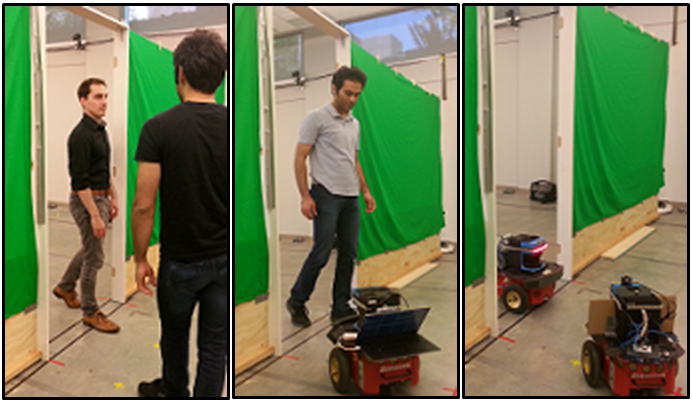
\includegraphics[scale=0.5]{Triptych.png}
      \caption{Examples of human-human, human-robot and robot-robot doorway interaction.}
      \label{fig:Triptych}
   \end{figure}

%\begin{figure}
%  \centering
%  \includegraphics[width=0.45\textwidth]{Robot_workplace}
%  \caption{Amazon staff work alongside a large multi-robot system, but their interactions are indirect and loosely coupled most of the time.}
%  \label{fig:Robot_workplace}
%\end{figure}

Our doorway negotiation behavior for autonomous robots navigating shared human-robot spaces is the main contribution of this paper. It is supported both by a robot-robot interaction experiment and by our non-expert user interaction study. The study also provides feedback on how the robot’s behavior was perceived by participants and how that perception influenced navigation performance.

\section{RELATED WORK}

Socially-compliant navigation for autonomous robots is a well-recognized interdisciplinary problem, touching on how robots navigate on their own, how humans and robots interact, and how past autonomy research has tried to use behavior to bridge that gap.

\subsection{Robot Navigation}

Navigation in general is one of the biggest topics in robotics research. Research on robot mobility often focuses on the physical dynamics and geometry of getting around as an entirely separate problem from social navigation, such as Fox et. al's Dynamic Window Approach to collision avoidance\cite{c2}. Other parties are often considered in the general form as ‘agents’, with no implicitly human characteristics, and whole complete robot systems can be built in this way. 

This might seem sufficient for domains that envision robots working alone or among themselves, but even when humans are not explicitly involved, models for robot navigation (particularly multi-agent ones) often take inspiration from human behavior. The Reciprocal Velocity Obstacle model proposed by van den Berg et. al\cite{c3} dealt with mutual collision avoidance for non-communicating agents by smooth, gradual trajectories where each agent assumes the other’s cooperation in ensuring a clean pass, directly citing an interest in "virtual human" behavior. 

This line of research has led to numerous extensions, such as Biased Reciprocal Velocity Obstacles\cite{c4} meant to alleviate congestion by building in more context sensitivity concerning who should defer to whom, or where Karamouzas et. al\cite{c5} turned the human-inspired model back toward humans to predict collision detection for a pedestrian simulator. Nevertheless, without explicitly designing for human interaction and studying how these behaviors are perceived in real life, these projects leave open the question of whether human-inspired necessarily equals human-compliant.


\subsection{Human-Robot Interaction}

HRI research into compliance for human-robot behavior has already explored some parts of the problem. Kretzschmar et. al\cite{c6} produced a model for training socially-compliant trajectories directly from datasets of human observation data, in explicit recognition that navigating human environments requires adaptation to human expectations. Shiomi et. al\cite{c7} acknowledge in their work that solving the obstacle avoidance problem for objects is insufficient when dealing with pedestrians, models must also include the higher problem of acceptable social distances. 

There is also evidence that humans are willing to reciprocate with robots that attempt to participate in social customs. Park et. al\cite{c8} found ``backchannel" signals from a listening robot in dialogue with a child would encourage that child to see the robot as more attentive to their story. For adults, a robot using recognizable gaze cues in conversation was found by Mutlu et. al\cite{c9} to provoke the correct social response in participants, seeing themselves as addressees or bystanders as appropriate. The takeaway is that the social acceptance of a robot necessary for its success may hinge on their behavior and how it is perceived.


\subsection{Autonomous Robot Behavior}

One assumption made here is that multi-robot systems introduced to human environments will be autonomous and governed by behaviors like the one we propose for doorway negotiation. When proposing design principles for autonomous agents\cite{c10}, Pfeifer described his "fungus eaters" as "systems capable of performing a set of tasks in the real world independently and without human intervention", able to deal with other robots, machines and humans while independently going about its business. These are all properties we may want for robots operating in shared human-robot spaces.

%It can be difficult to find a consistent, agreed-upon definition for autonomy, but Bekey suggests\cite{c10} ``Autonomy refers to systems capable of operating in the real-world environment without any form of external control for extended periods of time." This definition is broad, but it captures the benefit we articulated earlier of integrating robots into existing human (``real world") environments who are capable of holding up their end during social interactions without direct guidance(``external control"). 

Existing research on multi-robot systems in the workplace have often had these autonomous characteristics. The STRANDS project\cite{c11} is a sizable example where teams of robots are deployed to real office spaces for months at a time, with the stated goal of learning how to adapt and survive changes in the environment that would be fatally outside the scope of less independent robot systems. Dealing with humans around doorways is also an issue they encountered, but addressed only indirectly with passivity on the part of the robot, where humans near doors are treated as obstacles blocking them off.

These autonomous, distributed characteristics will also be present in the systems coming to share human spaces that we mentioned earlier. The self-driving car is the most obvious example, referred to almost interchangeably as the autonomous car in the popular press\cite{c12}. The conditions involved in driving – wide open spaces, large numbers of human and robot agents, the need to act quickly without guidance in network-denied environments – all necessitate an autonomous approach.


\section{SYSTEM OUTLINE}

The fundamental problem our behavior is meant to solve is when an autonomous robot wants to pass through a doorway and an interlocutor on the other side (whether another robot or a human) is trying to do the same, such that each blocks the path of the other. Our robot must be able to both make way when the other party approaches and vice-versa, as laid out in Figure~\ref{fig:Wireframe}. Since our interlocutor may be a human or human-controlled, we cannot assume the other party shares our robot’s programming or can communicate over the same network, so the interaction must be mediated through sensor interaction alone. We have chosen a previous robot-robot navigation behavior for distributed, autonomous robots as our starting point, as those constraints on communication and control closely match our own.

    \begin{figure}
      \centering
      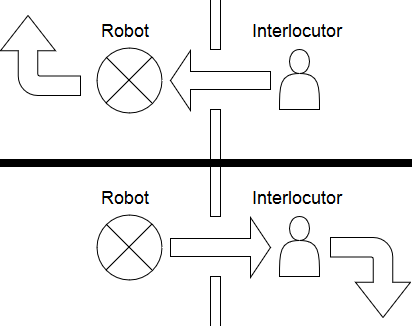
\includegraphics{wireframe.png}
      \caption{Sketch of outcomes for a doorway negotiating behavior to resolve}
      \label{fig:Wireframe}
   \end{figure}

\subsection{Preceding Approach - The Aggressive System}

Under the old method\cite{c1}, autonomous robots who approached one another in a corridor and found their paths mutually blocked would engage in a brief interaction to determine who would make way. Upon detecting each other, both robots would begin backing away until one robot achieves their desired ``safe distance". The more ``aggressive" the robot, the shorter this safe distance will be, where aggression level is a variable governed by the designer (e.g. distance from the robot’s goal).

On reaching its safe distance, the more aggressive robot would become ``brave" and start advancing toward the other robot, who would no longer be able to achieve their own safe distance until backing out of the corridor completely and allowing the aggressor to pass. A flowchart for this behavior can be seen in Figure~\ref{fig:Aggressive}.
 
    \begin{figure}
      \centering
      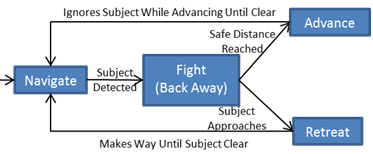
\includegraphics{aggressive_behavior.png}
      \caption{Outline of the Aggression System for Robot-Robot Corridor Interaction}
      \label{fig:Aggressive}
   \end{figure}
 
This system took deliberate inspiration from aggression displays in nature, used to assert dominance or divide resources. It was speculated at the time that it would also be compatible with humans, but this was not explicitly considered during the design process or evaluated with users. 


\subsection{Our Proposal - The Assertive System}

The behavior we propose will use the aggression system as a starting point, but shift the scenario to doorways rather than corridors. Changing the name from ``aggressive" to ``assertive" represents participating in polite human social etiquette but maintaining a willingness to assert the robot’s own right of way.

The first change is to govern when the robot becomes brave via time rather than distance, where the more assertive robot waits a shorter time before trying to advance. The robot also no longer backs up continuously after detecting the interlocutor, as to a human this might signal immediate deference. Instead, the robot takes only a half-step backward to show it has acknowledged the impasse but is waiting for a response. 

We must also address cases where interlocutors do not move if approached, or both parties decide to advance simultaneously. Our system will have a minimum distance which, if breached by the interlocutor while the robot is advancing, will cause the robot to stop. If the interlocutor backs away then the robot will resume advancing, otherwise the robot will wait a certain time (inversely proportionate to the time they waited before advancing, so that a more assertive robot will wait longer for an intransigent subject to move) before switching to retreating in hopes that the interlocutor will finally clear the way. A subject that cannot or will not clear the blocked doorway represents a problem beyond our scope. 
 
    \begin{figure}
      \centering
      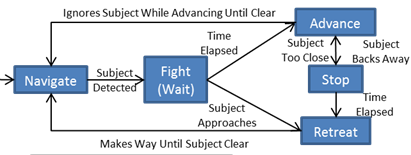
\includegraphics{assertive_behavior.png}
      \caption{Outline of the Assertive System for Negotiated Doorway Interaction}
      \label{fig:Assertive}
   \end{figure}
 


The final behavior flowchart can be seen in Figure~\ref{fig:Assertive}. While this describes the core interaction, it does not lay out what sort of feedback should be relayed or secondary sensor information integrated in a full implementation. As with the aggression system, this minimal description is meant to be generalizable to any mobile robot platform with the means to judge distance and discern subjects from the environment. Further information or signaling may enhance its performance, but first we must evaluate the fundamentals.


\section{EXPERIMENT AND STUDY}

Our behavior is presented as a socially compliant meant to solve navigation deadlocks around doors that humans can recognize and, through reciprocation, cooperate with to the benefit of the shared space. In order to test this theory, we have three hypotheses concerning our system that we evaluated through our robot-robot experiment and human-robot study:

\textbf{H1)} The assertive behavior resolves doorway navigation deadlocks for both human and robot agents.

\textbf{H2)} Overall performance of the behavior will be improved if humans respect the robot's right of way.

\textbf{H3)} Respecting the robot's right of way will correlate with recognizing their participation in a human social interaction.


\subsection{Setup}

Testing was divided into two discrete phases – one set of experimental robot-robot interactions, and one user study of human-robot interactions. It is important to note that the environment, robots, software and parameters were the same in both tests, as they would be in a live system.

The test environment for all experiments was a lab with a wall erected to divide the test space into two smaller rooms and with an open, standard-sized (97cm wide) doorway centered in it. Subjects in the smaller room would begin 2m from the door, while subjects in the larger room would begin 4m away. This ensured the closer party in each interaction should have right of way by arriving at the door first, as we would expect from two humans in this setting (all else being equal).

The robots used were Pioneer 3DXs, as seen in Figure~\ref{fig:Triptych}. Both were mounted with forward-facing range-finding lasers to provide navigational and detection data, using comparisons between a known map of the environment to determine if something in front is an obstacle or a possible interaction partner without distinguishing between different possible partners. They used rear-mounted sonars while retreating to avoid collisions. They had a top speed of 0.5m/s and stood 0.74m tall thanks to a paperwork-storing box used as part of the study, which gave them just enough physical presence to make stepping over them impractical but without posing a threat to participants.

Sensor data and user feedback were deliberately limited in this implementation to avoid distracting participants from evaluating the fundamental behavior. A strip of LEDs were mounted on the front of the Pioneer and would turn on when the behavior was active and turn off after arriving at its destination. These lights were green while traveling from the larger room to the smaller one and red on the return journey, which also corresponded to lower and higher assertiveness respectively, following our assumption about right of way. This basic feedback was included to see whether participants would correlate the color of the light with the assertiveness of the robot.


\subsection{Robot-Robot Experiment}

Each robot was set at their respective starting points either side of the doorway. At the beginning of each trial, the further robot would be given the instruction to drive to the other robot’s starting point, and after approximately one second the closer robot would receive the same instruction. This ensured the robot starting inside the smaller room would most likely reach the doorway first (with some variability on their exact meeting point) and was given the higher ``assertiveness" variable to reflect their expected right of way.

The desired outcome for each trial was that the more assertive, nearer robot would win the ensuing contest and have the other robot retreat until it could pass, whereupon the other robot would resume and finish its journey. Once both robots had reached their destinations, they would swap assertiveness values and goals and repeat the process. This was repeated 44 times, with the outcomes, interaction times and errors or other incidents recorded. 


\subsection{Human-Robot Study}

20 participants were recruited from the general population of Simon Fraser University, including 8 women and 12 men. They were not compensated for their assistance.

     \begin{figure}
      \centering
      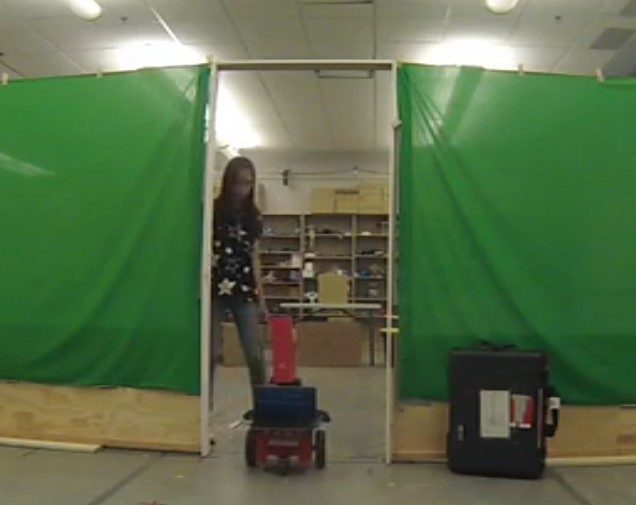
\includegraphics[scale=0.5]{test_example.png}
      \caption{A study participant deferring to the robot's right of way}
      \label{fig:Example}
   \end{figure}

Each participant was brought to the test environment and seated across from the test conductor in the smaller room, passing by the robot prepared for the experiment in the larger room. Every trial had the participant drop a document in a box in the larger room while the robot entered the smaller room to pick up some excess paperwork from the test conductor, then had the participant and robot return to their starting points. This created two interactions per trial, where we expected the human to have the right of way in the first part and the robot in the second. An example of a participant completing the study can be seen in Figure~\ref{fig:Example}. Each participant completed five trials:

\textbf{1) First Reaction Trial:} Without being informed as to the details of the experiment, the participant was asked to drop their signed consent form in a box on a table in the larger room, while the robot would be called in to collect the reusable part of the form. The participant incidentally interacted with the robot around the door as a result, and then again on their return journey. The participant was then informed that these incidental interactions were actually one of the trials, and the intent of the study was to examine their interactions with the robot around the doorway.

\textbf{2) Teleoperation Trial:} The participant was informed that the test conductor will take direct control of the robot via a controller, but to otherwise focus on the robot when deciding when to pass. 

\textbf{3) Full System Trial:} The participant was informed the full autonomous system would now be active and the test conductor would no longer be in control of the robot.

\textbf{4) Directed Behavior Trial:} For the first interaction, the participant was instructed to treat themselves as having absolute priority over the robot, and that the robot should defer to them. For the second, they were told to now treat the robot as having full priority, and that they should defer to it.

\textbf{5) Full Explanation Trial:} Before beginning the trial, the test conductor fully explained how the system worked to the participant, answering all questions until they were satisfied.

After each trial, the participant was given a survey to complete. These surveys contained four 5-point Likert Scale questions on the participant’s perception of the robot and the interaction during that trial. The survey questions were presented as statements with a scale ranging from strongly agree to strongly disagree, and are listed in Table 1.

\begin{table}[h]
\caption{Post-Trial Survey Questions}
\label{survey_questions}
\begin{center}
\begin{tabular}{|c|}
\hline
1) The robot’s intentions appeared clear.\\
\hline
2) The robot appeared to understand my intentions.\\
\hline
3) Our interaction went as smoothly as \\
it would have with another human.\\
\hline
4) The interaction was satisfactory overall.\\
\hline
\end{tabular}
\end{center}
\end{table}

Each survey also included a field for the participant to describe their account of what had happened during the trial and another field for additional comments. This form would be what the participant would drop off in the box in the large room for each trial.

Once all five trials were complete, a post-test questionnaire was administered by the test conductor, who transcribed the participant’s spoken responses. These questions are listed in Table 2.

\begin{table}[h]
\caption{Post-Test Questionnaire}
\label{questionnaire_questions}
\begin{center}
\begin{tabular}{|c|}
\hline
1) If or when you chose to press the robot, what \\
informed that decision in terms of signals you \\
were getting from the robot and your own motivations?\\
\hline
2) What about when you chose to defer to the robot?\\
\hline
3) In which trial do you think the interaction \\
worked best, in terms of getting where you \\
wanted to go and communicating between you and \\
the robot?\\
\hline
4) How would you compare these interactions to \\
those you have with other humans around doors?\\
\hline
5) What other behavior would you like to see from the robot? \\
What other feedback?\\
\hline
6) Any additional questions or observations.\\
\hline
\end{tabular}
\end{center}
\end{table}

\subsection{Results}

\textbf{1) Outcome:} The robot-robot interaction experiment had 44 trials, with 5 additional trials discounted due to navigational errors unrelated to our behavior. Of those 44, 40 trials completed as expected.  In four other cases, each robot first believed the other robot was approaching them and both retreated simultaneously, but they correctly resolved the interaction on the second attempt. All trials ended with the intended robot winning the interaction and both arriving at their desired destinations.

     \begin{figure}
      \centering
      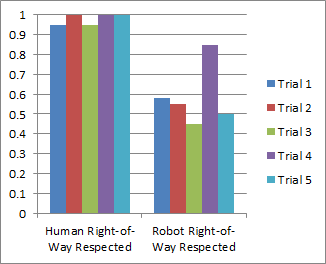
\includegraphics{outcomes.png}
      \caption{Outcomes Of Human-Robot Study Interactions Per Trial}
      \label{fig:Outcomes}
   \end{figure}

The outcome results for the human-robot interaction study are in Figure~\ref{fig:Outcomes}. The near-unanimous respect for the human's right of way in all trials when the participant was closest to the door demonstrated the interaction completed successfully without being too obtrusive or aggressive. Analyzing the second half of each trial revealed four discrete categories of participant: 

A) Those who would never respect the robot's right of way, sometimes even in trial 4 when specifically asked to. 

B) Those who did not respect the robot's right of way until the last trial then changed their behavior. 

C) Those who respected the robot's right of way until the last trial then changed their behavior. 

D) Those who always respected the robot's right of way. 

Our 20 participants were divided relatively evenly between these four categories, with five type A, four type B, five type C and six type D.
 
\textbf{2) Timing:} Our data from both the robot-robot experiment and human-robot study is collected in Figure~\ref{fig:Interaction} for time both subjects spent interacting during each trial and Figure~\ref{fig:Trial} for total time until both subjects reached their destinations, both with standard deviation error bars. In each trial, part 1 was the interaction where the human had right of way, while the robot had right of way in part 2. For context, one Pioneer making the 6m journey from one starting point to the other uninterrupted takes approximately 12 seconds.   
 

       \begin{figure}
      \centering
      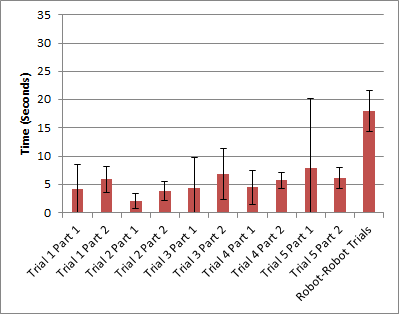
\includegraphics{interaction_length.png}
      \caption{Average Length Of Each Interaction In Each Trial}
      \label{fig:Interaction}
   \end{figure}


     \begin{figure}
      \centering
      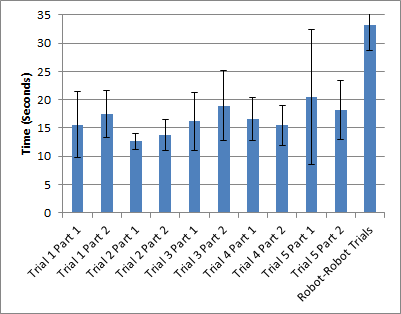
\includegraphics{trial_length.png}
      \caption{Average Length Of Each Trial}
      \label{fig:Trial}
   \end{figure}

The robot-robot behavior is much slower than any human-involved behavior. However, the human-robot interactions observed in the four non-teleoperated trials are only marginally slower than the interaction in the second trial, where a human is controlling the robot. This suggests that in terms of efficiency, our behavior is already be operating close to what may be possible for the given robot platform. Human interlocutors were able to compensate for the relatively cautious speed of the robot regardless of how it was being controlled. 

If we break down these time results according to our four participant behavior categories, seen in Figure~\ref{fig:Respect}, we found that participants who did not respect the robot's right of way had higher trial times than those who did across all trials. This reflects that while going out of turn might benefit the human individually, it degrades the throughput of the overall environment. 

     \begin{figure}
      \centering
      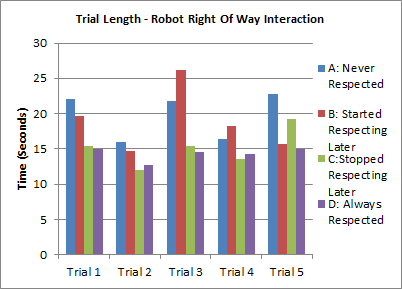
\includegraphics{Robot_right.png}
      \caption{Average Trial Length While Robot Had Right Of Way Per Participant Type}
      \label{fig:Respect}
   \end{figure}

\textbf{3) Surveys:} The data from the four Likert-scale questions on the post-trial surveys is collected in Figure~\ref{fig:Questionnaire}, with standard deviation error bars. The interaction was broadly positively received in each trial, but the slight bump for Q3 during trial 2 may suggest that having a known human operator controlling the robot was relevant to some participants. Similarly, some difficulty reading the robot's intentions in the very first interaction could have led to the relatively low Q1 score during trial 1.
 
     \begin{figure*}
      \centering
      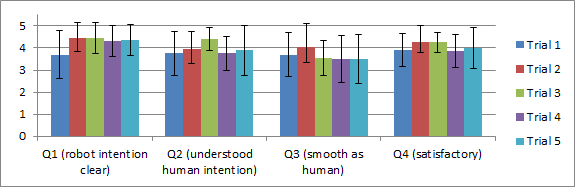
\includegraphics[width=\textwidth]{Questionnaire.png}
      \caption{Average Survey Score Per Trial Per Question }
      \label{fig:Questionnaire}
   \end{figure*}
 
Breaking down the scores according to our four participant categories did not produce a clear correlation between respecting the robot's right of way and a positive survey result. In fact, it was the type C and D participants in the first trial that gave low ratings for clear intentions and satisfaction. A participant who found they could make the robot back down in every confrontation may rate the interaction as satisfying as one who chose to respect the robot's right of way every time. Scores alone are not enough to distinguish different perceptions of the robot's behavior.

\textbf{4) Post-Test Questionnaire:} The questionnaire data was mostly qualitative, with the partial exception of question three where the participant gave their preferred trial. The overall results for this question are presented in Table 3 (with one abstention).

\begin{table}[h]
\caption{Number of Participants who Preferred Each Trial }
\label{Preferences}
\begin{center}
\begin{tabular}{|c||c|}
\hline
Trial One & 3\\
\hline
Trial Two & 4\\
\hline
Trial Three & 5\\
\hline
Trial Four & 3\\
\hline
Trial 5 & 4\\
\hline
\end{tabular}
\end{center}
\end{table}

Breaking down these preferences by our four participant behavior categories saw no significant correlation. Instead we found common justifications shared by participants who chose the same trial as their preference. All three participants who chose trial 4 cited that they preferred the decision on whether to defer to the robot or not be taken out of their hands, and similarly those who chose trial 2 mostly cited the speed of the interaction when the robot was being teleoperated. Participants who chose one of trials 1, 3 or 5 highlighted understanding the robot's intentions and the sense that it understood theirs, sometimes even directly referencing the humanlike characteristics of the behavior.

%The first two questions on the post-test questionnaire directly address why the participant would choose to advance or make way. Here we saw a difference between those who did and did not respect the robot's right of way, with those who did not predominantly phrasing their explanations in terms of efficiency - the robot was too slow, blocking their way. A smaller number believed they always had right of way, or that hesitation was an invitation to take the initiative. Some were curious what the robot would do if approached, and a few mentioned concerns that it might collide with them.

%By contrast, those who respected the robot's right of way often acknowledged that right as their reason. One mentioned buying into the premise of the study, assuming the robot might be carrying out some important work, and another suggested coworkers should be ``compatible". Curiosity was brought up, but also caution, concerned that they might damage or break the robot.

The first two questions on the post-test questionnaire directly address why the participant would choose to advance or make way. These responses were codified according to one of seven types, and the 20 answers to each question are presented in Table 4 and Table 5, grouped according to participant behaviour. The seven observed types of responses were:

\textit{Efficiency:} For the fastest resolution.

\textit{Right:} Acknowledged right of way.

\textit{Curiosity:} To see what would happen.

\textit{Safety:} To protect themselves or the robot.

\textit{Never:} Wouldn't do this.

\textit{Test:} Believed it was required by the test.

\textit{Learned:} In response to learning how the system worked in trial 5.

\begin{table}[h]
\caption{Cause For Advancing Toward Robot}
\label{Advance}
\begin{center}
\begin{tabular}{|c||c||c||c|}
\hline
\textbf{A} & \textbf{B} & \textbf{C} & \textbf{D}\\
\hline
Efficiency & Right & Learned & Safety\\
\hline
Efficiency & Curious/Test & Learned & Efficiency\\
\hline
Right & Speed & Curious & Right\\
\hline
Curious & Test & Efficiency & Efficiency\\
\hline
Right & & Curious & Curious\\
\hline
 & & & Right\\
\hline
\end{tabular}
\end{center}
\end{table}

\begin{table}[h]
\caption{Cause For Deferring To Robot}
\label{Defer}
\begin{center}
\begin{tabular}{|c||c||c||c|}
\hline
\textbf{A} & \textbf{B} & \textbf{C} & \textbf{D}\\
\hline
Safety & Safety & Right & Right\\
\hline
Right & Safety & Curious & Safety\\
\hline
Curious & Right & Curious & Right\\
\hline
Curious & Right & Right & Right\\
\hline
Never & & Right & Safety\\
\hline
 & & & Right\\
\hline
\end{tabular}
\end{center}
\end{table}

The number of participants who acknowledged the robot's right of way went from one among those who never deferred to four among those who always did. One type D participant mentioned buying into the premise of the study, assuming the robot might be carrying out some important work, and another suggested coworkers should be ``compatible". The difference could also be seen in the safety response, where type A and B participants cited concerns for their own safety, while type D participants were worried they could damage the robot. 

There were fewer differences between participants when comparing the interaction to those with other humans in the fourth question. The most common observation was that the robot was slower and less maneuverable than a human, and while some suggested the robot acted in a human-like manner it was couched as ``similar", yet still different.

Both the fifth question and the interaction accounts from the surveys produced a number of small implementation suggestions to smooth the interaction. Several participants noted that a human would know which direction to back up in order to clear their way faster, and others suggested that a human would speed up after noticing someone was already getting out of their way to minimize that person's delay. A few noted the Pioneer's wheels kept it from stepping briskly to the side the way a human might. Three participants described what was effectively a Reciprocal Velocity Obstacle interaction, where the robot cooperates at distance for a closer pass rather than one being forced to stop and back away from the other. 

\section{DISCUSSION}

\subsection{Hypotheses}

Our first hypothesis was that our behavior would resolve doorway navigation deadlocks, and in terms of both parties arriving at their destinations without incident that was the case in virtually all trials (a few unrelated navigation errors notwithstanding). Defined more narrowly, we found that our behavior executed as intended where the party with right of way was allowed to pass first in the vast majority of robot-robot trials and those human-robot interactions where the human had right of way. 

While most participants ignored the robot's right of way during at least one trial, 85\% could still complete the interaction as intended when asked to do so in trial 4. With that trial as a baseline, we can therefore say the behavior succeeded in resolving doorway deadlocks for both humans and robots, contingent on the cooperation of the human.

Our second hypothesis concerned whether respecting right of way increased overall performance, and average trial times showed  improvement for those who did. However, this measure of performance places the total throughput of a shared human-robot environment over the personal benefit of the individual human reaching their destination as soon as possible, a perspective the human may not share. This is not a problem unique to human-robot interaction, social behaviors in general could produce better outcomes but hinge on the acceptance of all participants.

This leads into our third hypothesis on whether those who respected the robot's right of way recognized the robot as participating in a human social interaction. The gap between respecting the robot's right of way in trial 4 and the other trials suggests the issue is not with the mechanics of the behavior. Gaining compliance is not something unique between humans, as participants were no more likely to respect the robot's right of way while it was being teleoperated than they were while it was controlled by our system. Few participants preferred the human-operated trial and none of those cited the human as the cause, while the "smooth as human" survey result for the teleoperation trial was only marginally higher than the rest.

The suggestions from the questionnaire and accounts on how to enhance the interaction demonstrated that participants were looking for more reciprocation from the robot for the social courtesies they extended, even if they did not recognize the robot's right of way. For those who did, they cast their decision to defer in terms of right and mutual concern. This contrasts with the accounts of those that did not, who emphasized speed, efficiency and the natural priority of humans. 

\subsection{Limitations}

As this method is meant to generalize to any ground robot it should be tested with other platforms beyond the Pioneer-3DX. It is likely that the exact form factor of the robot chosen had a significant effect on user perception of the behavior, and some performance shortfalls might be mitigated with more responsive movements and detections. 

The simple green/red LED signals also provoked very little participant interest. There was no evidence that participants distinguished between different levels of assertiveness or associated them with the different colors. Instead, several participants expressed a desire in the questionnaire for more indications of a robot’s intended action and direction, whether through subtle body language or explicit flashing lights, and a few thought the robot should simply say what it wanted aloud. 

\subsection{Future Work}

While we saw evidence that our system did provoke reciprocation from some participants, the large proportion who did not respect the robot's right of way shows that work remains in achieving acceptance. Establishing that perception of the robot as participating in human social interactions could help it achieve compliance and overall performance gives a goal to work toward, while participant feedback highlighted what additional behaviors would improve the experience.

Expanding the platform’s sensor capabilities could allow the system to integrate more nuanced information than distance when deciding when to act, like gestures or spoken commands. Though these capabilities were deliberately excluded to focus attention on the performance of the fundamental behavior, participant feedback emphasized the importance of picking up on smaller multi-modal cues to make the interaction more natural.

One avenue of exploration was revealed by accounts of the fifth trial. In some cases, particularly the type C participants who stopped respecting the robot's right of way in the last trial, hearing an explanation of how the behavior worked turned it into a mere mechanism rather than a social activity. Several chose to play with the robot, deliberately triggering the fight mechanism over and over to see if it would respond as predicted. Perhaps behavior development strategies that obscure the inner workings of a system, like machine learning, could impact human perception of that system.

\section{CONCLUSION}

This paper proposed an ``assertive" approach for robots to negotiate deadlocks at doors in a way compatible with both robots and humans. We tested our behavior with an experiment and a study, and found it resolved both robot-robot and human-robot impasses. Further, by examining what effect cooperation by humans had on performance and what provoked compliance, we found evidence that recognition of robot participation by humans may be an important part of successful social navigation.

Our system represents just one part of the larger pursuit of integrating human and robot environments. If we want to advance robots further into the public sphere where humans will be asked to share space with them, we should consider what the necessary conditions are for achieving coexistence.

\section*{ACKNOWLEDGMENT}

The authors would like to thank all participants for their assistance and the funding support of NSERC.

\begin{thebibliography}{99}

\bibitem{c0} Breazeal, Cynthia, and Brian Scassellati. ``How to build robots that make friends and influence people." \textit{Intelligent Robots and Systems, 1999. IROS'99. Proceedings. 1999 IEEE/RSJ International Conference on.} Vol. 2. IEEE, 1999.

\bibitem{c1} Zulaga, Maria, and Richard Vaughan. ``Reducing Spatial Interference in Robot Teams by Local-Investment Aggression", \textit{Proc. IEEE/RSJ Int. Conf. on Intelligent Robots and Systems}, Edmonton, Canada, 2005.

\bibitem{c2} Fox, Dieter, Wolfram Burgard, and Sebastian Thrun. ``The dynamic window approach to collision avoidance." \textit{IEEE Robotics & Automation Magazine} 4.1 (1997): 23-33.

\bibitem{c3} Van den Berg, Jur, Ming Lin, and Dinesh Manocha. ``Reciprocal velocity obstacles for real-time multi-agent navigation." \textit{Robotics and Automation, 2008. ICRA 2008. IEEE International Conference on}. IEEE, 2008.

\bibitem{c4} Sadat, Seyed Abbas, and Richard T. Vaughan. ``Bravo: Biased reciprocal velocity obstacles break symmetry in dense robot populations." \textit{Computer and Robot Vision (CRV), 2012 Ninth Conference on}. IEEE, 2012.

\bibitem{c5} Karamouzas, Ioannis, et al. ``A Predictive Collision Avoidance Model for Pedestrian Simulation." \textit{MIG} 9 (2009): 41-52.

\bibitem{c6} Kretzschmar, Henrik, et al. ``Socially compliant mobile robot navigation via inverse reinforcement learning." \textit{The International Journal of Robotics Research} 35.11 (2016): 1289-1307.

\bibitem{c7} Shiomi, Masahiro, et al. ``Towards a socially acceptable collision avoidance for a mobile robot navigating among pedestrians using a pedestrian model." \textit{International Journal of Social Robotics} 6.3 (2014): 443-455.

\bibitem{c8} Park, Hae Won, et al. ``Backchannel opportunity prediction for social robot listeners." \textit{Robotics and Automation (ICRA), 2017 IEEE International Conference on}. IEEE, 2017.

\bibitem{c9} Mutlu, Bilge, et al. ``Footing in human-robot conversations: how robots might shape participant roles using gaze cues." \textit{Proceedings of the 4th ACM/IEEE international conference on Human robot interaction}. ACM, 2009.

%\bibitem{c10} Bekey, George A. \textit{Autonomous robots: from biological inspiration to implementation and control}. MIT press, 2005.

\bibitem{c10} Pfeifer, Rolf. "Building fungus eaters: Design principles of autonomous agents." (1996).

\bibitem{c11} Hawes, Nick, et al. ``The strands project: Long-term autonomy in everyday environments." \textit{arXiv preprint}arXiv:1604.04384 (2016).

\bibitem{c12} https://www.economist.com/blogs/economist-explains/2015/07/economist-explains 

\end{thebibliography}

\end{document}
